\begin{center}
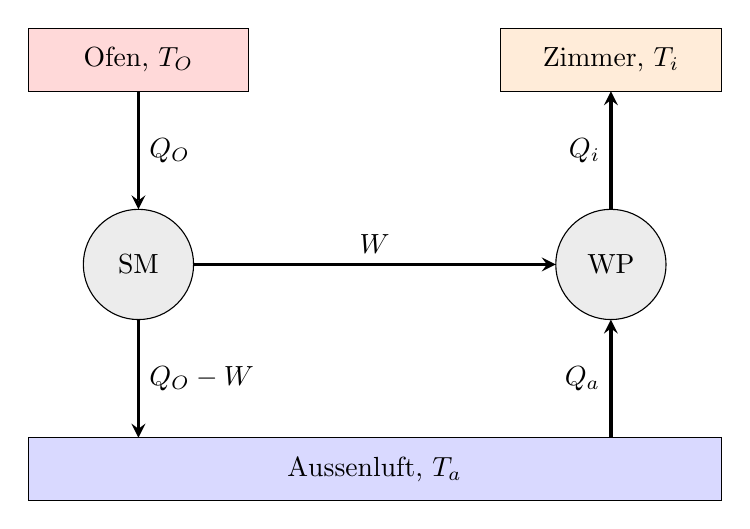
\begin{tikzpicture}[>=stealth]
 \draw[fill=red!15] (-4.4,2.2) rectangle (-1.6,3.0);
 \node at (-3,2.6) {Ofen, $T_\text{O}$};
 \draw[fill=orange!15] (1.6,2.2) rectangle (4.4,3.0);
 \node at (3,2.6) {Zimmer, $T_\text{i}$};
 \draw[fill=blue!15] (-4.4,-2.2) rectangle (4.4,-3.0);
 \node at (0,-2.6) {Aussenluft, $T_\text{a}$};
 \draw[fill=gray!15] (-3,0) circle (0.7);
 \node at (-3,0) {SM};
 \draw[fill=gray!15] (3,0) circle (0.7);
 \node at (3,0) {WP};
 \draw[->, very thick] (-3,2.2) -- (-3,0.7) node[midway, right] {$Q_\text{O}$};
 \draw[->, very thick] (-3,-0.7) -- (-3,-2.2) node[midway, right] {$Q_\text{O}-W$};
 \draw[->, very thick] (-2.3,0) -- (2.3,0) node[midway, above] {$W$};
 \draw[->, very thick] (3,-2.2) -- (3,-0.7) node[midway, left] {$Q_\text{a}$};
 \draw[->, very thick] (3,0.7) -- (3,2.2) node[midway, left] {$Q_\text{i}$};
\end{tikzpicture}
\end{center}

Die absoluten Temperaturen sind $T_\text{O} = \To$, $T_\text{a} = \Ta$ und $T_\text{i} = \Ti$. Gibt der Ofen die Wärme $Q_\text{O}$ an den Stirlingmotor ab, so verrichtet dieser mit dem Carnot-Wirkungsgrad die Arbeit
\begin{align}
 W &= \eta_\text{C}\,Q_\text{O}, \qquad \eta_\text{C} = \etSF = 1-\frac{\Ta}{\To} = \etS
\end{align}
Die ideale Wärmepumpe liefert damit die Wärme $Q_\text{i} = \eta_\text{WP}\,W$ ins Zimmer, mit
\begin{align}
 \eta_\text{WP} &= \ewpF = \frac{\Ti}{\Ti-\Ta} = \ewp
\end{align}
Im Verhältnis zur Wärme, die der Ofen allein ins Zimmer abgeben würde, ist das
\begin{align}
 \frac{Q_\text{i}}{Q_\text{O}} &= \eta_\text{C}\,\eta_\text{WP} = \fakF \\
   &= \etS\cdot\ewp = \fak \approx \result{\fakP{0}{2}}
\end{align}
$\result{\text{Ja}}$: Das System bringt rund viereinhalbmal so viel Wärme ins Zimmer wie der Ofen allein. Gibt man zusätzlich die Abwärme des Stirlingmotors statt an die Aussenluft ins Zimmer ab, wird es sogar noch besser.
